\documentclass{article}
%
%
%	groups.tex
%
%	David Meyer
%	dmm613@gmail.com
%	Last update: 24 Aug 2022
%
%
%   get various packages
%
\usepackage[margin=1.0in]{geometry}                                     % adjust margins
\geometry{letterpaper}                                                  % or a4paper or a5paper or ... 
\usepackage{url}                                                        % need this to use URLs in bibtex
\usepackage{setspace}                                                   % need this for \setstrech{...}
\usepackage{scrextend}                                                  % need this for addmargin
\usepackage[export]{adjustbox}                                          % need this to get frame for includegraphics
%
%   tikz et al
%
\usepackage{tikz}
\usetikzlibrary{calc,patterns,angles,quotes,shapes,math,decorations,
                through,intersections,lindenmayersystems,backgrounds}
\usepackage{circuitikz}                                                 % draw circuits    
\usepackage{pgfplots}
\usepackage{pgfplots}	
%
%	more math stuff
%
\usepackage{amsmath,amsfonts,amssymb,amsthm}
\usepackage{mathtools}
\usepackage{commath}                                                    % get \norm{x}
\usepackage{fixmath}                                                    % get \mathbold
\usepackage{gensymb}                                                    % get \degree
\usepackage{mathrsfs}
\usepackage{hyperref}
\usepackage{subcaption}
\usepackage{authblk}
\usepackage{graphicx}
\usepackage{hyperref}
\usepackage{alltt}
\usepackage{color}
\usepackage{float}
\usepackage{braket}
\usepackage{siunitx}
\usepackage{relsize}
\usepackage{multirow}
\usepackage{esvect}
%
%	watermarks
%
% \usepackage{draftwatermark}
% \SetWatermarkText{Draft}
% \SetWatermarkScale{5}
% \SetWatermarkLightness {0.9} 
% \SetWatermarkColor[rgb]{0.7,0,0}
%
%
%	theorems, definitions, etc
%
\theoremstyle{definition}
\newtheorem{theorem}{Theorem}[section]
\newtheorem{definition}{Definition}[section]
\newtheorem{proposition}{Proposition}[section]
\newtheorem{lemma}{Lemma}[section]
\newtheorem{example}{Example}[section]
\newtheorem{remark}{Remark}[section]
%
%	The following code allows you to do
%
%	\begin{bmatrix}[r] (or [c] or [l])
%
\makeatletter
\renewcommand*\env@matrix[1][c]{\hskip -\arraycolsep
  \let\@ifnextchar\new@ifnextchar
  \array{*\c@MaxMatrixCols #1}}
\makeatother
%
%	make \arg{min,max}_{n \to \infty} work nicely
%
\newcommand{\argmax}{\operatornamewithlimits{argmax}}
\newcommand{\argmin}{\operatornamewithlimits{argmin}}
%
%	handy commands
%
\newcommand*{\Scale}[2][4]{\scalebox{#1}{$#2$}}
\DeclareMathOperator{\E}{\mathbb{E}}
\DeclareMathOperator{\bda}{\Big \downarrow}
\newcommand{\veq}{\mathrel{\rotatebox{90}{$=$}}}
%
%	Title, author and date
%
\title{A Few Notes on Group, Ring and Field Theory}
\author{David Meyer \\ \href{mailto:dmm613@gmail.com}
                            {dmm613@gmail.com}}
\date{Last update: \today}
%
%
%
\begin{document}
\maketitle

\section{Introduction}
Group Theory is the study of symmetry. Symmetry takes many
different forms. Here we'll focus on the basic theory and use
that to motivate a few examples.

\section{Definitions}
The pair $(G,\circ)$ with the following four properties is called
a group: 

\begin{enumerate}
\item \textbf{Closure:} $x, y \in G \Rightarrow x \circ y \in G$
\\ In words: A group is closed under the group operation
$\circ$. $\circ$ is sometimes called "group multiplication" (or
even "multiplication") even though it might be some other
operation (such as addition).

\item \textbf{Associativity:} $x,y,z \in G \Rightarrow  (x \circ
y) \circ z = x \circ (y \circ z)$ 

\item \textbf{Identity:} $\exists e \in G \;  \text{s.t.} \;
\forall x \in G \; x \circ e = e \circ x = x$ 

\item \textbf{Inverse:} $\forall x \in G \;  \exists x^{-1} \in G
\;  \text{s.t.} \;  x \circ x^{-1} = x^{-1} \circ x = e$ 
\end{enumerate}

\bigskip
\noindent
The point here is that a group is a device that measures
symmetry.  

\bigskip
\noindent
Before doing an example, we need to define the \emph{order} of a
group element. Specifically, the order of a group
element\footnote{Not to be confused with the order of a group,
which for finite $G = \mid G \mid$.}  is the smallest integer
$n$, if it exists, such that $x^n = e$. Note that the
relationship between the order of an element and the order of a
group is that the order of the subgroup $\langle x \rangle$
generated by $x$ is $n$. That is, $x^n = e \Rightarrow | \langle
x \rangle | = n$.

\bigskip
\noindent
Now, consider the symmetries of a triangle shown in Figure
\ref{fig:symmetries_of_a_triangle}.  This forms a group called
$S_3$ where the group operation $\circ$ is function
composition. Here we name the vertices of the triangle with
"labels" from the set $\{1,2,3\}$. In this case our group has six
elements, as shown using cyclic notation in Table \ref{tab:s3}.

\bigskip
\begin{figure}
\center{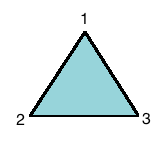
\includegraphics[scale=0.7] {images/s3.png}}
\caption{Symmetries of a Triangle}
\label{fig:symmetries_of_a_triangle}
\end{figure}


\bigskip
\begin{table}[H]
\centering
\begin{tabular}{c | |c| c | c | c }
Element & Type & Action & Inverse & Order \\
\hline
e       & No Op         & No Op                                 & e & 1 \\
(1 2)   & Reflection    & Fix 3, swap 1 \& 2                    & (1 2) & 2 \\
(2 3)   & Reflection    & Fix 1, swap 2 \& 3                    & (2 3) & 2 \\
(1 3)   & Reflection    & Fix 2, swap 1 \& 3                    & (1 3) & 2 \\
(1 2 3) & Rotation      & Rotate CW by $\frac{2 \phi}{3}$       & (1 3 2) & 3 \\
(1 3 2) & Rotation      & Rotate CCW by $\frac{2 \phi}{3}$      & (1 2 3) & 3
\end{tabular}
\caption{The Group $S_3$}
\label{tab:s3}
\end{table}

\noindent
A group is called \emph{Abelian} or \emph{commutative} if the
group operation $\circ$ commutes. That is, $\forall x,y \in G$ $x
\circ y = y \circ x$. Note that in our example above, $S_3$ is
not Abelian. You can see this if you consider: Let $x = (1 2)$
and $y = (2 3)$. Then $x \circ y \neq y \circ x$ since

\begin{flalign*}
(1 2) \circ (2 3) &= (1 2 3) \\
(2 3) \circ (1 2) &= (1 3 2) 
\end{flalign*}

\noindent
So $S_3$ is not Abelian. 

\bigskip
\noindent
One other example: Let $X$ be any set and $G =\{\text{bijections
} f: X \rightarrow X \}$ with group operation function
composition. Then $(G, \circ)$ is a group. To show this, we need
to show the following four things:

\begin{enumerate}
\item \textbf{Closure under $\circ$:} The composition of bijections 
			  is a bijection
\item \textbf{Associativity:} $(f \circ g) \circ h = f \circ (g \circ h)$
\item \textbf{Identity: } $I(x) = x$
\item \textbf{Inverse:} $y = f(x) \Leftrightarrow f^{-1}(y) = x$
\end{enumerate}


\bigskip
\noindent
One other definition we'll need here: A non-empty subset $H
\subseteq G$ is a \emph{subgroup}, denoted $H \leq G$, iff

\begin{enumerate}
\item \textbf{Closure:}  $x,y \in H  \Rightarrow x \circ y \in H$
\item \textbf{Inverses:} $x \in H \Rightarrow x^{-1} \in H$
\item \textbf{Identity:} $e \in H$  (implies $H$ non-empty)
\end{enumerate}

\section{Subgroups, Equivalence Relations, and Cosets}

Let $H \leq G$. $H$ induces an equivalence relation $\sim$ on $G$
as follows: For a group $G$, a subgroup $H \leq G$, and $x,y \in G$

\begin{equation}
x \sim y \; \text{iff} \; x = yh \;\text{for some}\;  h \in H
\label{eqn:er}
\end{equation}

\medskip
\noindent
The equivalence relation $\sim$ implies $H$ partitions $G$. We
define, for each $x \in G$, the \emph{equivalence class} of 
$x$, $E_{x}$, as


\begin{equation}
E_x = \{y \in G \mid x \sim y \}
\label{eqn:E_x}
\end{equation}

\medskip
\noindent
$E_x$ is sometimes denoted $[x]$.  In this case the notation $[x]
= \{y \in G \mid x \sim y\} \Rightarrow x^{-1}y \in H$ or $y \in
xH$. 

\bigskip
\noindent
Note that the $E_x$'s form a disjoint union: $\underset{x \in
G}{\cup} E_x = G$ and either $E_x = E_y$ or $E_x \cap \E_y =
\emptyset$ (this will become important later when we consider
Lagrange's Theorem (Theorem \ref{thm:lagrange})). 

\bigskip
\noindent
This is all good, but why does $x \sim y \Rightarrow x^{-1}y \in H$?
Here's one way to think about it:


\begin{equation*}
\begin{array}{llll}
x \sim y
&\Rightarrow& x = yh					&\hspace{4em} \mathrel{\#} 
												\text{definition of $\sim$ (Equation (\ref{eqn:er}))} \\
[3pt]
&\Rightarrow& x^{-1}x = x^{-1}yh		&\hspace{4em} \mathrel{\#} 
												\text{multiply both sides on the left by $x^{-1}$ 
												($x \in G \Rightarrow x^{-1} \in G$)} \\
[3pt]
&\Rightarrow& 1 = x^{-1}yh				&\hspace{4em} \mathrel{\#} x^{-1}x = 1 \\
[5pt]
&\Rightarrow& 1h^{-1} = x^{-1}yh h^{-1}	&\hspace{4em} \mathrel{\#} \text{multiply both sides on the right 
												by $h^{-1}$ ($h \in H \Rightarrow h^{-1} \in H$)} \\
[3pt]
&\Rightarrow& h^{-1} = x^{-1}y			&\hspace{4em} \mathrel{\#} 1h^{-1} = h^{-1},\; hh^{-1} = 1,
												\text{ and } (x^{-1}y)1 = x^{-1}y \\
[3pt]
&\Rightarrow& x^{-1}y \in H				&\hspace{4em} \mathrel{\#} \left [ \left ( h^{-1} \in H \right )  \, \land \, 
												\left ( h^{-1} = x^{-1}y \right ) \right ]  \Rightarrow x^{-1}y \in H
\end{array}
\end{equation*}

\smallskip
\noindent
So $x \sim y \Rightarrow x^{-1}y \in H$. $\blacksquare$

\bigskip
\noindent
By multiplying $x^{-1}y \in H$ on the left by $x$ we can state this conclusion 
in a slightly different form: 

\begin{equation*}
x \sim y \Rightarrow y \in xH
\end{equation*}

\medskip
\noindent
Here $xH = \{xh \mid h \in H\}$ for a fixed $x \in G$ and 
is called a \emph{left coset} of $H$ in $G$ for $x$. 

\bigskip
\noindent
Note that this also means that $E_x = xH$. To see this consider


\begin{equation*}
\begin{array}{llll}
E_x
&=& \{y \in G \mid x \sim y\}                           &\hspace{4em} \mathrel{\#} \text{definition of $E_x$ (Equation (\ref{eqn:E_x}))} \\
[3pt]
&=& \{y \in G \mid y \sim x\}                           &\hspace{4em} \mathrel{\#} \text{$\sim$ is symmetric:
															$x\sim y \Leftrightarrow y\sim x$} \\
[3pt]
&=& \{y \in G \mid y = xh \text{ for } h \in H\}		&\hspace{4em} \mathrel{\#} \text{definition of $\sim$ 
															(Equation (\ref{eqn:er}))} \\
[3pt]
&=& \{xh \in G \mid h \in H\}							&\hspace{4em} \mathrel{\#} y = xh \\
[3pt]
&=& \{xh \mid h \in H\}                                 &\hspace{4em} \mathrel{\#} \text{simplify} \\
[3pt]
&=& xH                                                  &\hspace{4em} \mathrel{\#} \text{definition of $xH$}\\
\end{array}
\end{equation*}

\smallskip
\noindent
So $E_x = xH$. $\blacksquare$

\bigskip
\noindent
Somewhat surprisingly $H$ and all of its cosets have the same
cardinality. That is, $|H| = |xH|\; \forall x \in G$.  The proof
of this is pretty straightforward. Here we just need to construct
a bijection $H \rightarrow xH$. We can do this by fixing a $x \in
G$ and considering $l_x: H \rightarrow xH$ by the map $h \mapsto
xh$. Then we need to show that $l_x$ is one-to-one and onto.

\begin{itemize}
\item one-to-one \\
For one-to-one we want to show that
$l_x(h_1) = l_x(h_2) \Rightarrow h_1 = h_2$. In this case we can
cancel on the left: $l_x(h_1) = l_x(h_2) \Rightarrow xh_1 = xh_2
\Rightarrow h_1 = h_2$.  So $l_x$ is one-to-one.
\item onto \\
Consider some $z \in xH$. Then $z = xh$ for some $h \in H$, so
$l_x(h) = z$ and therefore $l_x$ is onto. 
\end{itemize}

\medskip
\noindent
So $l_x: H \rightarrow xH$ is a bijection and therefore $H$ and
all of its cosets have the same cardinality, namely, $|H|$. 


\bigskip
\noindent
Here are a few useful definitions:

\medskip
\begin{itemize}
\item $| G |$ is the \emph{order} of $G$. If $G$ is finite then
      $|G| = \text{\# of elements in } G$. 
\item $| x |$ is the \emph{order} of $x$.  $|x|$ is the smallest
      positive integer $n$, if it exists, such that $x^n = e$. 
\item $[G:H]$ is the \emph{index} of $H$ in $G$. $[G:H] =
      \text{\# of cosets for $H$ (left or right) in $G$}$. 
\end{itemize}

\medskip
\noindent
With this machinery we can state and prove Lagrange's Theorem:

%\bigskip
\noindent
\begin{theorem}
\textbf{Lagrange's Theorem:}  Let  $G$ be a finite group and let
$H$ be a subgroup of $G$. Then $|H|$ divides $|G|$.  
\label{thm:lagrange}
\end{theorem}

\bigskip
\noindent
\textbf{Proof.} Recall that the left cosets of $H$ in $G$ form a
disjoint union of $G$. We also know that $|H| = |xH|$. Now suppose
that there are $k$ cosets.  Then $|G| = k |H|$. Since
$|G|$, $|H|$, and $k$ are integers we know that $|H|$ divides $|G|$. 
$\blacksquare$

\bigskip
\noindent
Note that if $G$ is finite, $[G:H] = \frac{|G|}{|H|}$. A nice
corollary of Lagrange's Theorem is that if $x \in G$ then $|x|$
divides $|G|$.

\section{Normal and Quotient Subgroups}
Let $G$ be any group. Then a subgroup $N \subseteq G$ is called
\emph{normal}, written $N \lhd G$, iff $\forall x \in G \; xN =
Nx$. Equivalently, $\forall x \in G \; N = xNx^{-1}$ (multiply on
the right by $x^{-1}$). Also equivalently $\forall x \in G \;
\forall n \in N \; x n x^{-1} \in N$. The last expression is
called conjugation by $x$.


\section{Group Actions}
The action of a group is a formal way of interpreting the manner
in which the elements of the group correspond to (usually linear)
transformations of some space in a way that preserves the
structure of that space. Common examples of spaces that groups
act on are sets, vector spaces, and topological spaces.  Actions
of groups on vector spaces are called representations of the
group (this is the subject of representation theory).

\bigskip
\noindent
\textbf{Definition:} An \emph{action} of the group $G$ on the set
$X$ is a map $G \times X \rightarrow X$ by $(g,x) \mapsto
\phi(g)x$ such that
\begin{itemize}
\item $\phi(e) x = x$
\item $\phi(g_1g_2) x = \phi(g_1) \big [ \phi(g_2)x \big ]$
\end{itemize}

\bigskip
\noindent
Examples of actions include 
\begin{itemize}
\item $G = (S_n$, $\circ$) and $X = \{1, \hdots, n\}$. Then for
      permutation $\sigma$, $\phi(\sigma)i = \sigma(i)$. \\ 
\item $G = (\mathbb{Z},+)$ and $X = \mathbb{R}$. Then the
      translations $\phi(n)x = x + n$ are an action. \\ 
\item $(S^1, +)$ and $X = \mathbb{C}$. Then the rotations
      $\phi(e^{i\theta})z = e^{i\theta}z$ are an action. 
\end{itemize}


\bigskip
\noindent
Another definition of group action is that we say that the group
$G$ acts on the set $X$ if there is a homomorphism $\phi: G
\rightarrow \text{Sym}(X)$.


\subsection{Group Actions and Equivalence Relations}
Perhaps surprisingly, it turns out that $x \sim y \Leftrightarrow
\exists g \in G \text{ s.t. } \phi(g)x = y$, where $\phi$ is as
defined above. So all the machinery developed for the equivalence
relations $E_x$ apply to actions, except that in the context of
group actions what we called equivalence classes above are called
orbits. Orbits are denoted $O_x$ and $O_x = E_x$.  In particular


\begin{flalign*}
O_x 
&= \{y \in X \mid x \sim y\} \\
&= \{ y \in X \mid \phi(g)x = y \} \\
&= \{\phi(g)x  \mid g \in G\}
\end{flalign*}

\smallskip
\section{Group Homomorphism}
Let $(G,\diamond)$ and $(H, \circ)$ be groups. Common usage is to
use $G$ to refer to $(G,\diamond)$. Similarly, $H$ will refer to
$(H, \circ)$. Then a mapping $\phi: G \rightarrow H$ is called a
\emph{homomorphism} iff

\medskip
\begin{equation*}
\phi(x \diamond y) = \phi(x) \circ \phi(y) \; \forall x,y \in G
\end{equation*}

\bigskip
\noindent
Essentially, a homomorphism $\phi: G \rightarrow H$ is a way of
exploring the structure of $H$ by varying $G$ using structure
preserving transformations. That is, $\phi$ preserves the group
operation.


\bigskip
\noindent
\textbf{Example:} Define a map

\begin{equation*}
\phi : G \rightarrow H
\end{equation*}

\bigskip
\noindent
where $G = \mathbb{Z}$ and $H = \mathbb{Z}_2 =
\mathbb{Z}/2\mathbb{Z}$ is the standard group of order two. Then
define $\phi: \mathbb{Z} \rightarrow \mathbb{Z}_2$ by the rule

\begin{equation*}
  \phi(x) =
    \begin{cases}
      0 & \text{if $x$ is even} \\
      1 & \text{if $x$ is odd}\\
    \end{cases}       
\end{equation*}

\bigskip
\noindent
It is easy to check that $\phi$ is a homomorphism. Suppose that
$x$ and $y$ are two integers. Then there are four cases:
\begin{itemize}
 \item $x$ and $y$ are both even
 
 In this case $\phi(x+y) = 0$ (even + even = even). Here
 $\phi(x)+\phi(y) = 0+0 = 0$ so $\phi(x+y) = \phi(x) + \phi(y) =
 0 + 0 = 0$.
 
 \item $x$ and $y$ are both odd
  
In this case $\phi(x+y) = 0$ (odd + odd = even).  Here $\phi(x) +
\phi(y) = 1 + 1 = 2 \mod 2 = 0$, so $\phi(x+y) = \phi(x) +
\phi(y) = 1 + 1 = 2 \mod 2 = 0$.

 \item $x$ is even and $y$ is odd or  $x$ is odd and  $y$ is even
 
In this case one is even and the other is odd and $x + y$ is odd.
Here $\phi(x+y) = 1$ and $\phi(x)+\phi(y) = 1+0 = 1$ so
$\phi(x+y) = \phi(x)+\phi(y)$.
 \end{itemize}
 
 \bigskip
 \noindent
Thus $\phi$ is a homomorphism. Note that in this example
$\diamond = +$ (normal addition in $\mathbb{Z}$) and $\circ = +$
(addition mod 2 in $\mathbb{Z}_2$).



\bigskip
\noindent
\textbf{Example:} Let $G = (\mathbb{R}, +)$ and $H =
(\mathbb{R}_{> 0}, \cdot)$ and let $\phi(x) = e^x$. To see that
$\phi$ is a homomorphism consider $\phi(x + y)$:

\begin{equation*}
\begin{array}{rcll}
\phi(x + y) 
&=& e^{(x + y)}          
		&\hspace{8em} \mathrel{\#} \text{definition of $\phi$} \\
[3pt]
&=& e^x e^y
		&\hspace{8em} \mathrel{\#} a^{(b + c)} = a^b a^c \\
[3pt]
&=& \phi(x) \phi(y)
		&\hspace{8em} \mathrel{\#} \text{definition of $\phi$} \\
[3pt]
&=& \phi(x) \phi(y)
		&\hspace{8em} \mathrel{\#} \phi(x + y) = \phi(x) \phi(y) 
		 \Rightarrow \text{$\phi$ is a homomorphism}
\end{array}
\end{equation*}

\bigskip
\noindent
Note that in this example $\diamond = +$ (normal addition) and
$\circ = \cdot$ (normal multiplication).  

\bigskip
\noindent
Frequently the group operation is the same for $G$ and $H$ (like,
for example, if $\phi: G \rightarrow G$). So in many cases we see
the homomorphism property expressed as follows:

\begin{equation*}
\phi(xy) = \phi(x)\phi(y) \; \forall x,y \in G
\end{equation*}

\bigskip
\noindent
\textbf{Example:} Let $G$ be a group with $N \lhd G$ ($N$ is a
normal subgroup of $G$). Define the \emph{quotient homomorphism}
$q$ as

\begin{equation*}
q: G \rightarrow  G/N 
\end{equation*}

\bigskip
\noindent
and let $x \mapsto xN$ by $q(x) = xN$. To show that $q$ is a
homomorphism, let $x,y \in G$ and consider $q(xy)$:


\begin{equation*}
\begin{array}{rcll}
q(xy) 
&=& xyN                 &\hspace{5em} \mathrel{\#} \text{definition of $q$} \\
[5pt]
&=& xyNN                &\hspace{5em} \mathrel{\#} NN =N \text{ for $N$ a subgroup in $G$} \\
[5pt]
&=& x (yN) N            &\hspace{5em} \mathrel{\#} \text{group multiplication is associative} \\
[5pt]
&=& x (Ny) N            &\hspace{5em} \mathrel{\#} \text{$N$ normal so  $xN = Nx$} \\
[5pt]
&=& (xN)(yN)            &\hspace{5em} \mathrel{\#} \text{group multiplication is associative} \\
[5pt]
&=& q(x) q(y)           &\hspace{5em} \mathrel{\#} \text{definition of $q$} \\
[5pt]
&=& q(x) q(y)			&\hspace{5em} \mathrel{\#} q(xy) = q(x) q(y) \Rightarrow \text{$q$ is a homomorphism} 
\end{array}
\end{equation*}


\bigskip
\begin{lemma}
Let $G$ and $H$ be groups where $e$ is the identity in $G$ and
$f$ is the identity in $H$ and define a homomorphism $\phi: G
\rightarrow H$. Then
\begin{enumerate}
\item $\phi(e) = f$. That is,  $\phi$ maps the identity in $G$ to
      the identity in $H$. \item $\phi(a^{-1}) = (\phi(a))^{-1}$. That is, 
      $\phi$ maps inverses to inverses.
\item If $K$ is a subgroup of $G$ then $\phi(K)$ is a subgroup of $H$.
\end{enumerate}
\label{lemma:homomorphism}
\end{lemma}

\bigskip
\noindent
\textbf{Proof.} To show 1. in Lemma \ref{lemma:homomorphism},
first let $a = \phi(e)$. Then

\begin{equation*}
\begin{array}{rcll}
a 
&=& \phi(e)
                &\hspace{13em} \mathrel{\#}  \text{by assumption} \\
[5pt]
&=& \phi(e \cdot e)
                &\hspace{13em} \mathrel{\#} x \cdot e = e \cdot x = x \text{ so } e = e \cdot e \\
[5pt]
&=& \phi(e) \cdot \phi(e)
                &\hspace{13em} \mathrel{\#} \text{$\phi$ is a homomorphism}\\
[5pt]
&=& a \cdot \phi(e)
                &\hspace{13em} \mathrel{\#} a = \phi(e)  \text{ (by assumption)} \\
[5pt]
&=& a \cdot a
                &\hspace{13em} \mathrel{\#} \hdots \\
[5pt]
&\Rightarrow& a \cdot a^{-1} =  (a \cdot a)  \cdot a^{-1}
                &\hspace{13em} \mathrel{\#} \text{multiply on the right by  $a^{-1}$} \\
[5pt]
&\Rightarrow& a \cdot a^{-1} =  a \cdot (a \cdot a^{-1})
                &\hspace{13em} \mathrel{\#} \text{multiplication is associative} \\
[5pt]
&\Rightarrow& a \cdot a^{-1} =  a \cdot  f
                &\hspace{13em} \mathrel{\#} a \cdot a^{-1} = f, 
                 \text{ where $f$ is the identity in $H$} \\
[5pt]
&\Rightarrow& a \cdot a^{-1} =  a
                &\hspace{13em} \mathrel{\#} a \cdot  f  = a \\
[5pt]
&\Rightarrow& f = a
                &\hspace{13em} \mathrel{\#} a \cdot a^{-1} = f  \text{ by definition of inverse} \\
[5pt]
&\Rightarrow& \phi(e) =  f
                &\hspace{13em} \mathrel{\#} \text{$\phi$ maps the identity in $G$ to the identity in $H$}
\end{array}
\end{equation*}

\bigskip
\noindent
So $\phi$ maps the identity in $G$ to the identity in $H$ which
shows 1. $\blacksquare$

\bigskip
\noindent
Another approach is to recognize that if the group operation is
$+$, then $0$ is the (additive) identity, that is, $0 + x = x + 0
= x$. Then

\begin{equation*}
\begin{array}{rcll}
0 + x 
&=& x                                                           &\quad \mathrel{\#} \text{$0$ is the additive identity} \\
&\Rightarrow& \phi(0  + x) = \phi(x)                            &\quad \mathrel{\#} \text{apply $\phi$} \\
&\Rightarrow& \phi(0) +  \phi(x) = \phi(x)                      &\quad \mathrel{\#} \phi \text{ is a homomorphism} \\
&\Rightarrow& (\phi(0) + \phi(x)) - \phi(x) = \phi(x) -\phi(x)  &\quad \mathrel{\#} \text{subtract $\phi(x)$ from both sides} \\
&\Rightarrow& (\phi(0) + \phi(x)) - \phi(x) = 0                 &\quad \mathrel{\#} \phi(x) -\phi(x) = 0 \\
&\Rightarrow& \phi(0) + (\phi(x) - \phi(x)) = 0                 &\quad \mathrel{\#} \text{addition is associative} \\
&\Rightarrow& \phi(0) + 0  = 0                                  &\quad \mathrel{\#} \phi(x) -\phi(x) = 0 \\
&\Rightarrow& \phi(0) = 0                                       &\quad \mathrel{\#} \phi(x) \text{ maps $0$ to $0$}
\end{array}
\end{equation*}

\bigskip
\noindent
So $\phi(0) = 0$. A similar argument can be used where the group
operation is multiplication: 

\begin{equation}
\begin{array}{rcll}
1 \cdot x 
&=& x
                &\quad \mathrel{\#} \text{$1$ is the multiplicative identity} \\
&\Rightarrow& \phi(1 \cdot x) = \phi(x)
                &\quad \mathrel{\#} \text{apply $\phi$} \\
&\Rightarrow& \phi(1) \cdot \phi(x) = \phi(x)
                &\quad \mathrel{\#} \phi \text{ is a homomorphism} \\
&\Rightarrow& (\phi(1) \cdot \phi(x)) \cdot  (\phi(x))^{-1} =
\phi(x) \cdot  (\phi(x))^{-1}
                &\quad \mathrel{\#} \text{multiply on the right by $ (\phi(x))^{-1}$} \\
&\Rightarrow& (\phi(1) \cdot \phi(x)) \cdot  (\phi(x))^{-1} = 1
                &\quad \mathrel{\#}\phi(x) \cdot  (\phi(x))^{-1}  = 1 \\
&\Rightarrow& \phi(1) \cdot (\phi(x) \cdot  (\phi(x))^{-1}) = 1
                &\quad \mathrel{\#} \text{multiplication is associative} \\
&\Rightarrow& \phi(1) \cdot 1 = 1
                &\quad \mathrel{\#} \phi(x) \cdot  (\phi(x))^{-1} = 1 \\
&\Rightarrow&  \phi(1) = 1
                &\quad \mathrel{\#}  x \cdot 1 = x
\end{array}
\label{eqn:1}
\end{equation}

\bigskip
\noindent
So we have $\phi(0) = 0$ and  $\phi(1) = 1$. 

\bigskip
\noindent
To show 2., note that since $G$ is a group, $x^{-1} \in G$ and
$x \cdot x^{-1} = 1$ for $x, x^{-1}  \in G$. Then 

\begin{equation}
\begin{array}{rcll}
 x \cdot x^{-1}
&=& 1                                           &\hspace{8em} \mathrel{\#} \text{definition of inverse} \\
&\Rightarrow& \phi(x \cdot x^{-1}) = \phi(1)    &\hspace{8em} \mathrel{\#} \text{apply $\phi$} \\
&\Rightarrow& \phi(x \cdot x^{-1}) = 1          &\hspace{8em} \mathrel{\#} \phi(1) =1 \text{(Equation (\ref{eqn:1}))} \\
&\Rightarrow& \phi(x) \cdot \phi(x^{-1}) = 1	&\hspace{8em} \mathrel{\#} \phi \text{ is a homomorphism} \\
&\Rightarrow& \phi(x^{-1}) = 1/\phi(x)			&\hspace{8em} \mathrel{\#} \text{divide both sides by } \phi(x) \\
&\Rightarrow& \phi(x^{-1}) = (\phi(x))^{-1}		&\hspace{8em} \mathrel{\#} \text{hence $\phi$ maps inverses to inverses}
\end{array}
\label{eqn:inverse}
\end{equation}

\bigskip
\noindent
Finally, to show 3., let $X = \phi(K)$. Then it suffices to show
that $X$ is non-empty and closed under products and inverses. $X$
contains $f$, the identity of $H$, by 1.  above. We also know
that $X$ is closed under inverses by 2. above. Finally, we know
that $X$ and is closed under products (almost) by
definition. Thus $X$ is a subgroup.  $\blacksquare$

\begin{theorem}
Let $G$ and $H$ be groups and let $f: G \rightarrow H$ be a group
homomorphism. Then $f$ is one-to-one iff the kernel of $f$ is
trivial, that is, $\ker f = \{e\}$ where $e$ is the identity
element of $G$.
\end{theorem}

\noindent
\textbf{Proof.}  Here we'll show that $f$ is one-to-one  $\iff
\ker f =\{e\}$:  
\begin{itemize}
\item $f$ is one-to-one  $\Rightarrow \ker f =\{e\}$ 

Suppose the homomorphism $f : G \rightarrow H$ is
one-to-one. Then since $f$ is a group homomorphism, the identity
element $e$ of $G$ is mapped to the identity element $e^\prime$
of $H$. That is, $f(e ) = e^\prime$ (see Equation (\ref{eqn:1})
above).

Now let $g \in \ker f$, so $f(g) = e^\prime$, recalling that
$\ker f = \{g \in G \mid f(g) = e^\prime\}$. So now $f(e) =
e^\prime$ and $f(g) = e^\prime$ which implies that $f(g)=f(e)$.
 
Since $f$ is one-to-one\footnote{Recall that saying $f$ is
one-to-one means that $f(x) = f(y) \Rightarrow x = y$.} we know
that $f(g) = f(e) \Rightarrow g = e$, so $g = e$. But $g$ was an
arbitrary element of $\ker f$ so $f$ maps every $g \in \ker f$ to
$e$. Hence $\ker f = \{e\}$.

\item $\ker f = \{e\} \Rightarrow f$ is one-to-one

On the other hand, suppose that $\ker f = \{e\}$ and that there
exists $g_1, g_2 \in G$ such that

\begin{equation}
f(g_1) = f(g_2) 
\label{eqn:g}
\end{equation}

Now consider an element $g_1g_2^{-1} \in G$. Then

\begin{equation}
\begin{array}{rcll}
f(g_1g_2^{-1})
&=& f(g_1) f(g_2^{-1})          &\hspace{7em} \mathrel{\#} \text{$f$ is a homomorphism} \\
&=& f(g_1) (f(g_2))^{-1}        &\hspace{7em} \mathrel{\#} f(g_2^{-1})   = (f(g_2))^{-1}
														\text{ (Equation (\ref{eqn:inverse}))} \\
&=& f(g_1) (f(g_1))^{-1}        &\hspace{7em} \mathrel{\#} f(g_2) = f(g_1)  \text{ (Equation (\ref{eqn:g}))} \\
&=& e^\prime                    &\hspace{7em} \mathrel{\#} f(g_1) (f(g_1))^{-1}  = e^\prime
\end{array}
\label{eqn:eprime}
\end{equation}

So $f(g_1g_2^{-1}) = e^\prime$ which implies that $g_1g_2^{-1}
\in \ker f$. But by assumption $\ker f = \{e\}$ so $g_1g_2^{-1} =
e$.

If you multiply $g_1g_2^{-1}  = e$  on the right by $g_2$, you
notice that  

\begin{equation*}
\begin{array}{rcll}
g_1g_2^{-1}
&=& e                                                           &\hspace{3em} \mathrel{\#} \text{Equation (\ref{eqn:eprime})} \\
&\Rightarrow&  (g_1 \cdot g_2^{-1}) \cdot g_2 = e \cdot g_2     &\hspace{3em} \mathrel{\#} \text{multiply on the right by $g_2$} \\
&\Rightarrow&  g_1 \cdot  (g_2^{-1} \cdot g_2) = e \cdot g_2    &\hspace{3em} \mathrel{\#} \text{multiplication is associative} \\
&\Rightarrow&  g_1 \cdot e = e \cdot g_2                        &\hspace{3em} \mathrel{\#} g_2^{-1} \cdot g_2 = e \\
&\Rightarrow&  g_1 =  g_2                                       &\hspace{3em} \mathrel{\#} e \cdot g = g \cdot e = g
\end{array}
\end{equation*}


So $f(g_1) = f(g_2)$ (Equation (\ref{eqn:g})) implies that 
$g_1 = g_2$ and so $f$ is one-to-one.
\end{itemize}

\noindent
This shows that $f$ is one-to-one  $\iff \ker f =\{e\}$. 
$\blacksquare$

\section{The First Isomorphism Theorem}
The First Isomorphism Theorem (FIT) is a handy piece of machinery
for many problems in group theory. Before getting to all of that,
recall the following:

\smallskip
\begin{itemize}
\item $\phi: G \rightarrow G^\prime$ is called a
      \textbf{group homomorphism} if it preserves the group 
      operation: $\phi(ab) = \phi(a)\phi(b)$.
\item The \textbf{image of $\mathbf{G}$:}  $\phi(G) = \{\phi(g) \mid g \in G\}$.
\item The \textbf{kernel of $\boldsymbol{\phi}$}: $\ker \phi =
      \{g \in G \mid \phi(g) = e^\prime\}$  ($e^\prime$ is the identity
      in $G^\prime$). 
\item $\phi(a) = \phi(b)$ iff $a \ker \phi = b \ker \phi$.
\item If $\phi(g) = g^\prime$ then $\phi^{-1}(g^{\prime}) = g
      \ker \phi$. 
\end{itemize}

\medskip
\noindent
So here's a theorem:

\medskip
\begin{theorem}
	Let $\phi: G \rightarrow H$ be a  group
	homomorphism. Then $\ker \phi  \lhd  G$.
\label{theorem:kernel_is_a_normal_subgroup}
\end{theorem} 


\medskip
\noindent
{\bf Proof: }To prove the theorem, first let $k \in \ker \phi$ 
and let $g \in G$. Then we want to show\footnote{Recall that for 
normal subgroups $xN = Nx$ which implies that $xnx^{-1} \in N$.}  
that $gkg^{-1} \in \ker \phi$ (or equivalently that 
$g \ker \phi \, g^{-1} = \ker \phi$). Now consider $\phi(gkg^{-1})$:

\begin{equation*}
\begin{array}{rcll}
\phi(gkg^{-1})
&=& \phi(g)\phi(k)\phi(g^{-1})
                &\hspace{8em} \mathrel{\#} \text{$\phi$ is a homomorphism} \\
[5pt]
&=& \phi(g)\phi(k)(\phi(g))^{-1}
                &\hspace{8em} \mathrel{\#} \text{Equation (\ref{eqn:inverse}): }\phi(g^{-1}) = (\phi(g))^{-1} \\
[5pt]
&=& \phi(g) e_H (\phi(g))^{-1}
                &\hspace{8em} \mathrel{\#} k \in \ker \phi \Rightarrow \phi(k) = e_H  
                				\text{ ($e_H$ is the identity in $H$)} \\
[5pt]
&=& \phi(g) (\phi(g))^{-1}
                &\hspace{8em} \mathrel{\#} \phi(g) e_H = \phi(g) \text{ and } 
                				e_H \phi(g)^{-1} = \phi(g)^{-1} \\
[5pt]
&=& e_H
                &\hspace{8em} \mathrel{\#} xx^{-1} = x^{-1} x = e_H 
                				\text{ (where $x \in H$ and $x \neq 0$)} \\
[5pt]
&=& e_H
                &\hspace{8em} \mathrel{\#} \phi(gkg^{-1}) = e_H \Rightarrow 
                				gkg^{-1} \in \ker \phi
\end{array}
\end{equation*}


\noindent
So $gkg^{-1} \in \ker \phi \Rightarrow g \ker \phi \, g^{-1} =
\ker \phi \Rightarrow \ker \phi \lhd G$. $\blacksquare$


\medskip
\noindent
\begin{example}
Consider the group $(\mathbb{Z}_{12},+)$ and
let $\phi: \mathbb{Z}_{12} \rightarrow \mathbb{Z}_{12}$ by
$\phi(x) = 3x$.
\end{example}

\medskip
\noindent
To show that $\ker \phi \lhd (\mathbb{Z}_{12},+)$, we first need
to show that $\phi$ is a homomorphism. But this is an easy one:
$\phi(x+y) = 3 (x + y) = 3x + 3y = \phi(x) + \phi(y)$.  So $\phi$
is a homomorphism. Next consider the mapping $\phi$ on
$\mathbb{Z}_{12}$:


\begin{equation*}
\begin{array}{l c c c c c c c c c c c c}
\mathbb{Z}_{12}:  & 0    & 1    & 2    & 3    & 4    & 5    & 6    & 7    & 8    & 9    & 10   & 11 \\
                  & \bda & \bda & \bda & \bda & \bda & \bda & \bda & \bda & \bda & \bda & \bda & \bda \\
\phi(x):          & 0    & 3    & 6    & 9    & 0    & 3    & 6    & 9    & 0    & 3    & 6    & 9 \\
\end{array}
\end{equation*}

\bigskip
\noindent
We can see that the image of $\mathbb{Z}_{12}$,
$\phi(\mathbb{Z}_{12}) = \{0,3,6,9\}$ and that $\ker \phi =
\{0,4,8\}$.    

\bigskip
\noindent
Grouping the  elements of $\mathbb{Z}_{12}$ with their images we 
see that 


\medskip
\begin{equation*}
\begin{array}{l c c c c}
\mathbb{Z}_{12}: & \{0,4,8\}     & \{1,5,9\}   & \{2,6,10\}  & \{3,7,11\} \\
                 & \bda          & \bda        & \bda        & \bda \\
\phi(x):         & 0             & 3           & 6           & 9 \\
                 & \bda          & \bda        & \bda        & \bda \\
\phi(x)^{-1}:    & \{0,4,8\}     & \{1,5,9\}   & \{2,6,10\}  & \{3,7,11\} \\
                 & \veq          & \veq        & \veq        & \veq \\
                 & 0 + \ker \phi & 1+\ker \phi & 2+\ker \phi & 3+\ker \phi

\end{array}
\end{equation*}

\bigskip
\noindent
This is a nice example of the group property that $\phi(a) = x
\Rightarrow \phi^{-1}(x) = a \circ \ker \phi$. In this case the
group operation $\circ$ is $+$. To see this how this works,
choose, for example, $a = 5$. Then $\phi(5) = 3\cdot 5 = 15$ and
$15 \operatorname{mod} 12 = 3$, so $x = 3$. This implies that
$\phi(3)^{-1} = 5 + \ker \phi = \{5+0, 5+4, 5+8\} = \{5, 9, 13\}
\equiv \{1,5,9\}$, noting that $13 \operatorname{mod} 12 = 1$.

\bigskip
\noindent
Now we can state the First Isomorphism Theorem:

\medskip
\begin{theorem} {\bf First Isomorphism Theorem:}
Let
$\phi: G \rightarrow H$ be an onto homomorphism.  Then $H \simeq
G/N$, where $N = \ker \phi$.
\end{theorem}

\medskip
\noindent
Though somewhat technical this is really an amazing theorem. 
So here's one way to prove the theorem: construct an isomorphism
$\widetilde{\phi}: G/N \rightarrow H$ by 
$\widetilde{\phi}(gN) = \phi(g)$. To show this, we need to 
demonstrate three things: (i). that $\widetilde{\phi}$ is 
well-defined, (ii). that $\widetilde{\phi}$ is a homomorphism, 
and (iii). that $\widetilde{\phi}$ is one-to-one and onto.

\begin{itemize}
\item To show that $\widetilde{\phi}$ is
well-defined\footnote{Well-defined is kind of the opposite of
one-to-one where we show that if $f(x) = f(y)$ then $x = y$.}
we need to show that if $gN = hN$ then $\widetilde{\phi}(gN) =
\widetilde{\phi}(hN)$. Now, if $gN = hN$ then since $N$ is the
the identity in $G/N$, $g = hn$ for some $n \in N$. This means

\begin{equation*}
\begin{array}{rcll}
\widetilde{\phi}(gN)
&=& \phi(g)                                     &\hspace{8em} \mathrel{\#} \text{definition of $\widetilde{\phi}(gN)$} \\
[3pt]
&=& \phi(hn)                                    &\hspace{8em} \mathrel{\#} g = hn \text{ since } gN = hN \text{ by assumption} \\
[3pt]
&=& \phi(h)\phi(n)                              &\hspace{8em} \mathrel{\#} \text{$\phi$ is a homomorphism} \\
[3pt]
&=& \phi(h)e                                    &\hspace{8em} \mathrel{\#} n \in N = \ker \phi = \{x \in G  \mid \phi(x) = e\} \\
[3pt]
&=&  \phi(h)                                    &\hspace{8em} \mathrel{\#} x \cdot e = x \\
&=& \widetilde{\phi}(hN)                        &\hspace{8em} \mathrel{\#} \text{definition of $\widetilde{\phi}$} \\
[3pt]
\widetilde{\phi}(gN) &=& \widetilde{\phi}(hN)   &\hspace{8em} \mathrel{\#} \text{so $\widetilde{\phi}$ is well-defined}
\end{array}
\end{equation*}

\item Next, we need to show that $\widetilde{\phi}$ is a
      homomorphism. To see this, consider  

\begin{equation*}
\begin{array}{rcll}
\widetilde{\phi}(gN hN)
&=& \widetilde{\phi}(ghNN)
                &\hspace{3em} \mathrel{\#} \text{definition of group multiplication} \\
[3pt]
&=& \widetilde{\phi}(ghN)
                &\hspace{3em} \mathrel{\#} NN = N \text{($N$ a subgroup)} \\
[3pt]
&=& \phi(gh)
                &\hspace{3em} \mathrel{\#} \text{definition of $\widetilde{\phi}$} \\
[3pt]
&=& \phi(g)\phi(h)
                &\hspace{3em} \mathrel{\#} \phi \text{ is a homomorphism} \\
[3pt]
&=& \widetilde{\phi}(gN) \widetilde{\phi}(hN)
                &\hspace{3em} \mathrel{\#} \text{definition of $\widetilde{\phi}$} \\
[3pt]
\widetilde{\phi}(gN hN) &=& \widetilde{\phi}(gN)
\widetilde{\phi}(hN)
                &\hspace{3em} \mathrel{\#} \text{therefore $\widetilde{\phi}$ is a homomorphism}
\end{array}
\end{equation*}

\medskip
\noindent
So $\widetilde{\phi}$ is a homomorphism.

\item For one-to-one, we need to show that $\widetilde{\phi}(gN)
= \widetilde{\phi}(hN) \Rightarrow gN = hN$. We know that if
$\widetilde{\phi}(gN) = e_H$, then $\phi(g) = e_H$. So $g \in
\ker \phi$ (recalling that $N = \ker \phi$). This implies that
$gN \in N$ ($N$ is the identity in $G/N$). Similarly for
$\widetilde{\phi}(hN)$, so $\widetilde{\phi}$ is one-to-one. [ed:
this isn't complete]

\item Finally, to show onto, choose a $h$ in $H$. We want to show
that $\exists gN \in G/N \text{ with } \widetilde{\phi}(gN) =
h$. Well, we know that $\phi$ is onto so $\exists g \in G$ with
$\phi(g) = h$. This means that $\widetilde{\phi}(gN) = \phi(g) =
h$, so $\widetilde{\phi}$ is onto.
\end{itemize}


\smallskip
\noindent
This shows that $H \simeq G/\ker \phi$. $\blacksquare$

\section{Rings, Ideals and Homomorphisms}
This section provides a few notes on Ring Theory. To start, a few
definitions 

\noindent
\begin{definition}
A ring $R$ is an abelian group with a multiplication operation  
\begin{equation*} (a, b) \mapsto ab \end{equation*} which is 
associative and satisfies the distributive laws $a(b+c) = ab+ac$ 
and $(a+b)c = ac+bc$ and has identity element 1.
\end{definition}

\noindent
Here there is a group structure with the addition operation but
not necessarily with the multiplication operation. Thus an
element of a ring may or may not be invertible with respect to
the multiplication operation.

\begin{definition}
Let $a,b$ be in a ring $R$. If $a \neq 0$ and $b \neq 0$ but $ab
= 0$, then we say that $a$ and $b$ are \emph{zero divisors}. If
$ab = ba = 1$, we say that $a$ is a \emph{unit} or that $a$ is
invertible.
\end{definition}

\noindent
For example, consider the ring $\mathbb{Z}_n$. Notice that if $n$
is not prime then $\mathbb{Z}_n$ has zero divisors. For a
concrete example, consider the ring $\mathbb{Z}_{10}$ and let $a
= 2$ and $b = 5$. Then $ab = 2 \cdot 5 = 10$ and $10 \operatorname{mod} 
10 = 0$, so 2 and 5 are zero divisors in $\mathbb{Z}_{10}$. On the
other hand, if $n = p$ is prime then the only factors of $p$ are
1 and $p$, so $\mathbb{Z}_p$ has no zero divisors.

\begin{definition}
Let $R$ be a ring. Then if $ab = ba$ for any $a,b \in R$ then $R$
is said to be \emph{commutative}. 
\end{definition}

\noindent
In general, for a given ring $R$ the addition operation is
commutative, but the the multiplication operation may or may not
be commutative.  There are two particular kinds of rings where
the multiplication operation is well-behaved:

\begin{definition}
An \emph{integral domain} is a commutative ring with no zero
divisors. A \emph{division ring} or skew field is a ring in which
every non-zero element $a$ has an inverse $a^{-1}$.
\end{definition}

\noindent
For example, the integers $\mathbb{Z}$ form an integral
domain. The quaternions (more on this later) form a division
ring. 

\begin{definition}
The characteristic of a ring $R$, denoted by $\text{char}(R)$, is
the smallest positive integer $n$ such that 

\begin{equation*}
n \cdot 1 = \underbrace{1 + 1 + \cdots + 1}_{n \text{ times}} = 0
\end{equation*}
\end{definition}


\bigskip
\noindent
One more definition then we'll look at a few examples.

\begin{definition}
A subring of a ring $R$ is a subset $S$ of $R$ that forms a ring
under the operations of addition and multiplication defined in
$R$. 
\end{definition}

\subsection{Examples}
Before diving into examples, it is worthwhile to notice that the
concepts of subrings and ideals, while related, have subtle and
important differences.  Both an ideal $I$ and a subring $S$ of a
ring $R$ are subsets of $R$ which are subgroups under addition
and are closed under multiplication. However, each has an
additional property:

\begin{itemize}
\item An ideal $I$ has the absorption property ($\forall r \in R$
$rI \subset I$), while a subring is only required to be closed
under multiplication.
\item A subring $S$ is usually required to contain the
multiplicative identity 1, while an ideal is not required to
contain 1. 
\end{itemize}

\noindent
For example, consider the integers $\mathbb{Z}$.  $\mathbb{Z}$ is
a subring of the rational numbers $\mathbb{Q}$ but is not an
ideal since $\frac{1}{2} \cdot 1 = \frac{1}{2}$ and $\frac{1}{2}
\notin \mathbb{Z}$ (that is, $\mathbb{Z}$ does not \emph{absorb}
$\mathbb{Q}$). On the other hand, the subset $2\mathbb{Z} \subset
\mathbb{Z}$, where $2\mathbb{Z} = \{2n \mid n \in Z\}$ is an
ideal of $\mathbb{Z}$ but is not a subring (since $1 \notin
2\mathbb{Z}$). A few other examples:

\begin{itemize}
\item $\mathbb{Z}$ is an integral domain but not a field since
      only $\{-1,1\}  \in \mathbb{Z}$ have inverses in $\mathbb{Z}$. 
\item As we saw above, the integers modulo $n$, $\mathbb{Z}_n$,
      form a ring which is an integral domain if and only if $n$ is
      prime. 
\item The $n \times n$ matrices $\mathcal{M}_{n}(\mathbb{R})$
      with coefficients in $\mathbb{R}$ are a ring, but not an 
      integral domain if $n \geq 2$.
\item The quaternions are the smallest and perhaps the most
      famous example of a division ring. To see this, first take
      $1, i, j, k$ to be basis vectors for a 4-dimensional vector
      space over $R$, and define multiplication by 

\begin{flalign*}
i^2     &= j^2 = k^2 = -1, \\
ij      &= k, \\
jk      &= i, \\
ki      &= j, \\ 
ji      &= -ij, \\
kj      &= -jk, \\
ik      &= -ki
\end{flalign*}

\noindent
Then we can define the quaternions $\mathbb{H} = \{a + bi + cj +
dk, \text{ for } a,b,c,d \in R \}$. $\mathbb{H}$ forms a division
ring called the quaternions \cite{horn2001}.  To show that
$\mathbb{H}$ is a division ring, we need to show that every
non-zero element is invertible. To do this, consider the
\emph{conjugate} of an element $h = a + bi + cj +dk \in H$ to be
$\bar{h} = a - bi - cj - dk$; note that this is analogous to the
complex conjugates we saw for complex numbers in $\mathbb{C}$.
It is pretty easy to see (multiply it out) that

\begin{equation*}
q\bar{q} = a^2 + b^2 + c^2 + d^2 
\end{equation*}

\noindent
Next,  take 
\begin{equation}
q^{-1} = \frac{q}{q \bar{q}}
\label{eqn:quat}
\end{equation}

\bigskip
\noindent
Then  $qq^{-1} = q^{-1}q = 1$ and the denominator in Equation
\ref{eqn:quat} cannot be $0$ unless $a = b = c = d = 0$. 
\end{itemize}

\bigskip
\noindent
As we saw with groups, we can define a map from a ring to another
which has the property of carrying one ring structure to the
other. 

\bigskip
\begin{definition}
Let $R$ and $S$ be rings. A map $f : R \rightarrow S$  satisfying
\begin{enumerate}
\item $f(a + b) = f(a) + f(b)$  (so $f$ is a group homomorphism under +)
\item $f(ab) = f(a)f(b)$
\item $f(1_R) = 1_S$
\end{enumerate}
for $a, b \in R$ is called \emph{ring homomorphism}
\end{definition}

\subsection{Ideals}
The concept of an "ideal number" was introduced by the
mathematician Kummer as being some special numbers (well, today
we call them groups) having the property of unique factorization,
even when considered over more general rings than
$\mathbb{Z}$. Today's definition of \emph{ideals} looks more
like:

\begin{definition}
Let $I$ be a subset of a ring $R$. Then an additive subgroup of
$R$ having the property that 

\medskip
\begin{equation*}
ra \in I \text{ for }  a \in I, \: r \in R
\end{equation*}

\medskip
\noindent
is called a left ideal of $R$.  Similarly

\medskip
\begin{equation*}
ar \in I  \text{ for }  a \in I, \: r \in R
\end{equation*}

\bigskip
\noindent
is called a right ideal of $R$. If an ideal is both a right and a
left ideal then we call it a two-sided ideal of $R$, or simply an
ideal of $R$. 
\end{definition}

\noindent
We say that an ideal $I$ of $R$ is proper if $I \neq R$.  We say
that is it non-trivial if $I \neq R$ and  $I \neq  0$. 

\bigskip
\noindent
I've seen several different notations for ideals including, among
others:  $rI = \{ri \mid r \in R, i \in I\}$ and $rI \subset I \;
\forall r \in R$.  

\bigskip
\noindent
So in words: An ideal $I$ is a subset of a ring $R$ such that

\begin{itemize}
\item $I$ is a subgroup of $R$ under addition (so $0 \in I$ and
      so $I \neq \emptyset$)  
\item $I$ is not only closed under multiplication but also
      satisfies the \emph{stronger property} that it "absorbs"
      all of the elements of $R$ under multiplication: $\forall r
      \in R$ $rI \subset I$ 
\end{itemize}

\bigskip
\noindent
In addition, if $f : R \rightarrow S$ is a ring homomorphism we
define the kernel of $f$ in the expected way, namely, $\ker f =
\{r \in R \mid f(r) = 0\}$. Since a ring homomorphism is a group
homomorphism, we already know that $f$ is one-to-one iff $\ker f
= \{0\}$.  $\ker f$ is a proper two-sided ideal since

\begin{itemize}
\item $\ker f$ is an additive subgroup of $R$
\item Take $a \in \ker f$ and $r \in R$. Then $f(ra) = f(r)f(a) =
      0$ and $f(ar) = f(a)f(r) = 0$ so both $ra$ and $ar$ are in 
      $\ker f$. 
\end{itemize}

\noindent
Quick proof: Since $\ker f$ is a two-sided ideal of $R$, then
either $\ker f = \{0\}$ or $\ker f = R$.  But $ker f \neq R$
since $f(1) = 1 $ by definition. In words, $\ker f$ is a proper
ideal.

\bigskip
\noindent
It is worth noticing the analogy between rings and their
two-sided ideals and groups and their normal subgroups: 

\begin{itemize}
\item Two-sided ideals are stable when the ring acts on them by
      multiplication, either on the right or on the left, and so 
\begin{equation*}
rar^{-1} \in I \text{ for }a \in I \text{ and } r \in R
\end{equation*}

\noindent
while normal subgroups are stable when the groups act on them on
them by conjugation: 
\begin{equation*}
ghg^{-1} \in H \text{ for } h \in H, g \in G
\end{equation*}

\noindent
That is  $H \lhd G$.
\item Groups with only trivial normal subgroups are called
      simple. We will not see it formally here, but rings with
      only trivial two-sided ideals as in the above lemma are
      called simple rings.
\item The kernel of a group homomorphism is a normal subgroup,
      while the kernel of a ring homomorphism is an ideal. 
\item Normal subgroups allowed us to define quotient groups. We
      will see now that two-sided ideals will allow to define
      quotient rings. 
\end{itemize}

\subsection{Quotient rings}
Let I be a proper two-sided ideal of $R$. Since $I$ is an
additive subgroup of $R$ by definition, it makes sense to speak
of cosets $r + I$ of $I$ where $r \in R$. Furthermore, a ring has
a structure of abelian group for addition, so $I$ satisfies the
definition of a normal subgroup.  From group theory we know that
of the quotient group is
\begin{equation*}
R/I = \{r + I \text{ for } r \in R\}
\end{equation*}
%
%
%
\bigskip
\section*{Acknowledgements}
Thanks to Joel Bion for pointing out a typo in an early version
of these notes. 
%
%	LaTeX source on overleaf.com
%
\section*{\LaTeX \hspace{0.10 mm} Source}
\url{https://www.overleaf.com/read/xjmnmzvrgsfk}
%
%	get a bibliography
%
%	Note:.bib files go in ~/Library/texmf/bibtex/bib with TeXShop (MacTeX).
%	You can also use an absolute path, e.g. \bibliography{/Users/dmm/papers/bib/qc}
%
\bibliographystyle{plain}
\bibliography{qc}
%
%	done
%
\end{document} 

